% =====================================================================
%  Compile with:  pdflatex week3_report_revised.tex
%  (run it twice so references resolve)
%  Optional: run vonkarman_response.jl first to generate the result plot.
% =====================================================================
\documentclass[11pt]{article}

\usepackage[margin=1in]{geometry}
\usepackage{amsmath, amssymb}
\usepackage{graphicx}
\graphicspath{ {./imgs/} } 
\usepackage{tikz}
\usepackage{kotex}
\usepackage{booktabs}
\usepackage[hidelinks]{hyperref}
\usetikzlibrary{decorations.pathmorphing, patterns, arrows.meta}
\usepackage{appendix}
\usepackage{verbatim}

\title{\textbf{Wing Vibration as a Low-Pass Filter:\\
A Two-Degree-of-Freedom Typical-Section Model\\
under von K\'arm\'an Gust Excitation}}
\author{C417025 김세경}
\date{\today}

\begin{document}
\maketitle
\begin{comment}
\begin{abstract}
\noindent
This report examines whether an aircraft wing, when buffeted by atmospheric turbulence,
behaves as a low-pass filter with resonant peaks at low frequency. To answer
this at a tractable level, the wing is reduced to a rigid \emph{typical
section} with two degrees of freedom---plunge and pitch---supported by two
spring--damper units. The turbulent forcing is supplied by the von K\'arm\'an
vertical-gust spectrum. We derive the equations of motion from energy
principles, obtain the gust-to-response transfer function, and show that the
measured output spectrum is the product of the input spectrum and the squared
transfer function. Dividing one by the other isolates the wing's own dynamic
behaviour, which is approximately flat at low frequency, resonant near the two
natural frequencies, and rolling off above them---the signature of a low-pass
filter.
\end{abstract}
\end{comment}

% =====================================================================
\section{Introduction}
% =====================================================================
A wing in cruise is continuously excited by turbulence: wake disturbances,
clear-air turbulence, and the broadband ``aperiodic'' eddies advected past it
by the freestream. Physically, the wing is expected to respond strongly to slow
disturbances, to amplify those near its natural frequencies, and to ignore very
fast disturbances that its inertia cannot follow. This behaviour is precisely a
low-pass filter with resonant peaks.

Resolving the turbulence itself with computational fluid dynamics is expensive
and unnecessary for this question because the filtering is a property of the
\emph{structure}, not of the detailed flow physics. We therefore adopt the
classical typical-section idealisation \cite{hodges2011,fung1955}: the wing is treated
as a rigid airfoil on elastic supports, retaining only the two motions that
matter for bending- and torsion-like responses. Turbulence enters as a
prescribed gust velocity with the statistics of the von K\'arm\'an model
\cite{vonkarman1948}.

% =====================================================================
\section{The Model}
% =====================================================================
Figure~\ref{fig:airfoil_diagram} shows the model\cite{hodges2011,fung1955}. A rigid airfoil with chord $c_{\text{chord}}$ and span
$b$ rests on two identical supports, each a spring of stiffness $k$ in parallel
with a damper of coefficient $c$, separated by a distance $d$. We place the
reference point at the midpoint between the supports and describe the motion using

\begin{itemize}
\item[] $h$ --- the \emph{plunge}, vertical displacement of the reference point
(positive downward), and
\item[] $\theta$ --- the \emph{pitch}, rotation of the section (positive
nose-up).
\end{itemize}

A chordwise material point a distance $\xi$ \emph{aft} of $P$ moves downward by
\begin{equation}
z(\xi) = h + \xi\,\theta ,
\label{eq:kin}
\end{equation}
since a nose-up rotation ($\theta>0$) lowers points behind $P$ and raises points ahead of it. The centre of gravity lies a distance $x_{\mathrm{cg}}$ \emph{aft} of the
reference, and the aerodynamic centre a distance $e_a$\footnote{$e_a=x_{\mathrm{cg}}-x_{\mathrm{ac}}$} \emph{forward} of it. These two offsets are the only sources of coupling between $h$ and $\theta$.

\begin{figure}[ht]
\centering
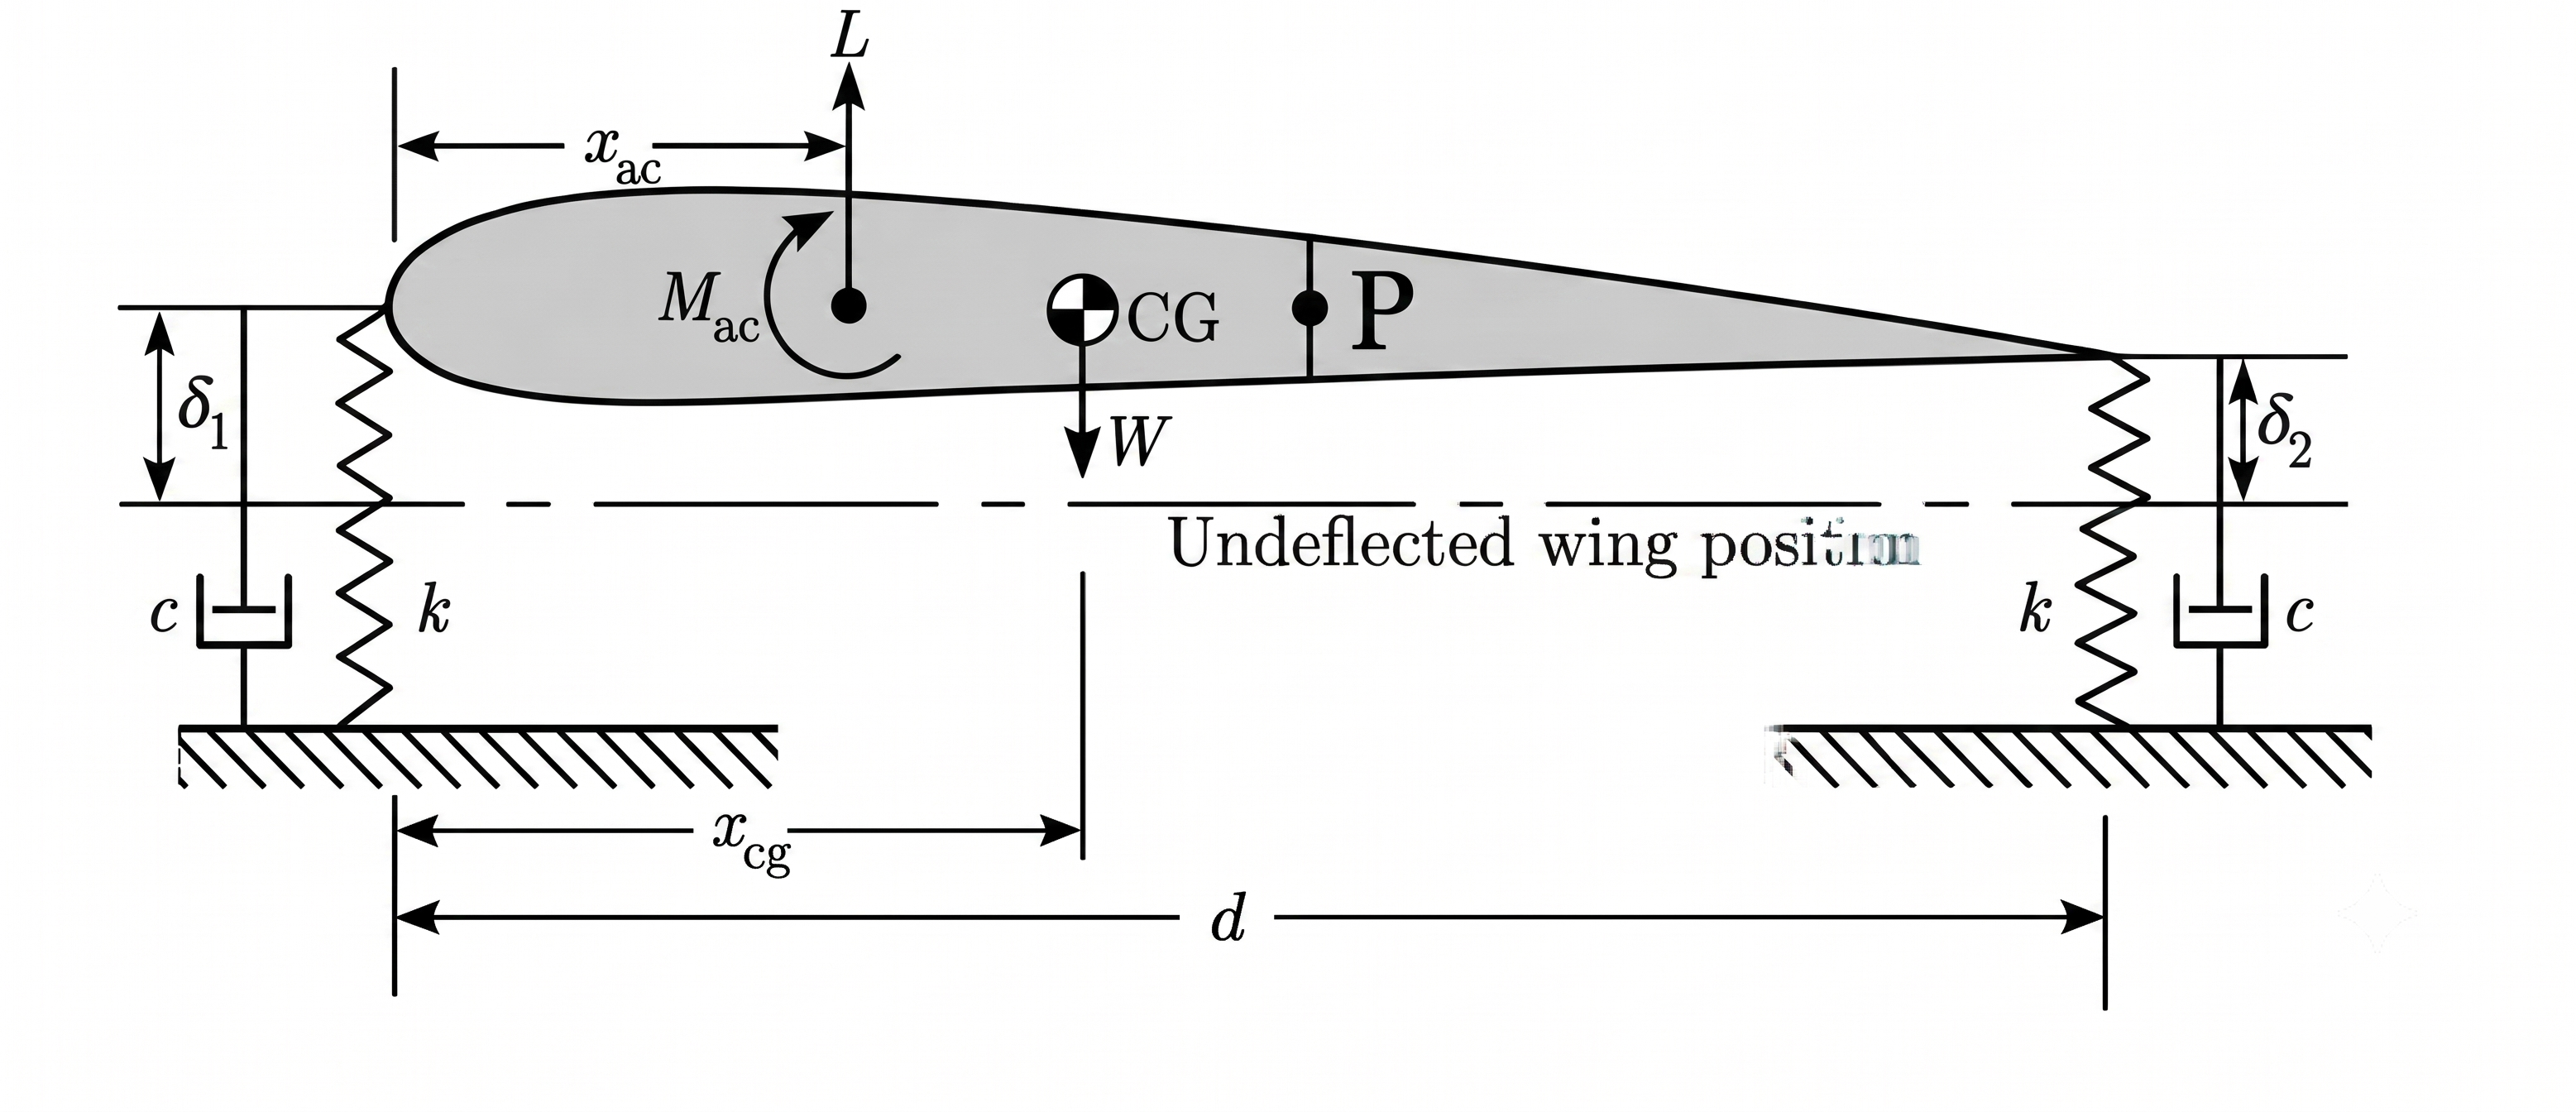
\includegraphics[width=0.85\textwidth]{model_diagram.png}
\caption{Typical-section model. The wing is represented as a rigid airfoil on two
spring--damper supports, with two degrees of freedom: plunge $h$ and pitch
$\theta$. Lift $L$ acts at the aerodynamic centre, and weight $W$ acts at the centre of
gravity.}
\label{fig:airfoil_diagram}
\end{figure}

%======================================================================
\section{Structural Model from Energy}
%======================================================================

\subsection{Mass Matrix --- Kinetic Energy}
Let the section have mass $m$, centre of gravity a distance $x_{\mathrm{cg}}$ aft
of $P$, and moment of inertia $I_{\mathrm{cg}}$ about the c.g. From \eqref{eq:kin}, the
downward velocity of the c.g. is $\dot z_{\mathrm{cg}}=\dot h + x_{\mathrm{cg}}\dot\theta$,
so the kinetic energy is
\begin{equation}
T = \tfrac12 m\,(\dot h + x_{\mathrm{cg}}\dot\theta)^2 + \tfrac12 I_{\mathrm{cg}}\dot\theta^2
  = \tfrac12 m\dot h^2 + S\,\dot h\dot\theta + \tfrac12 I_p\,\dot\theta^2 ,
\label{eq:T}
\end{equation}
where the \textbf{static unbalance} and \textbf{inertia about $P$} are defined as
\begin{equation}
S \equiv m\,x_{\mathrm{cg}}, \qquad I_p \equiv I_{\mathrm{cg}} + m\,x_{\mathrm{cg}}^2 .
\end{equation}
Writing $T=\tfrac12\dot{\mathbf q}^{\mathsf T}\mathbf M\dot{\mathbf q}$ with
$\mathbf q=[\,h,\ \theta\,]^{\mathsf T}$ gives
\begin{equation}
\boxed{\;\mathbf M=\begin{bmatrix} m & S\\[2pt] S & I_p \end{bmatrix}\;}
\label{eq:M}
\end{equation}
The off-diagonal $S$ represents the \emph{inertial coupling}: if the c.g. is not at $P$, plunge and
pitch exchange energy. Setting $x_{\mathrm{cg}}=0$ decouples them.

\subsection{Stiffness Matrix --- Spring Potential Energy}
The two springs sit at $\xi=-d/2$ (front) and $\xi=+d/2$ (rear). Their deflections are
$z_{1}=h-\tfrac{d}{2}\theta$ and $z_{2}=h+\tfrac{d}{2}\theta$, so
\begin{equation}
V=\tfrac12 k z_1^2+\tfrac12 k z_2^2
 =\tfrac12 k\!\left[\Big(h-\tfrac d2\theta\Big)^2+\Big(h+\tfrac d2\theta\Big)^2\right]
 = k\,h^2+\tfrac14 k d^2\,\theta^2 .
\label{eq:V}
\end{equation}
The cross terms $\mp d\,h\theta$ cancel because $P$ is the midpoint. With
$V=\tfrac12\mathbf q^{\mathsf T}\mathbf K_s\mathbf q$,
\begin{equation}
\boxed{\;\mathbf K_s=\begin{bmatrix} 2k & 0\\[2pt] 0 & \tfrac12 k d^2 \end{bmatrix}\;}
\label{eq:Ks}
\end{equation}
i.e., plunge stiffness $2k$ and pitch stiffness $\tfrac12 kd^2$.

\subsection{Damping Matrix --- Rayleigh Dissipation}
The dampers act in parallel with the springs, so the Rayleigh dissipation function is
identical in form to \eqref{eq:V} with $k\!\to\!c$ and $z\!\to\!\dot z$:
$\mathcal D=\tfrac12 c\dot z_1^2+\tfrac12 c\dot z_2^2$, giving\footnote{For a viscous damper $F_{v}=c\dot{z}$, the Rayleigh dissipation function is $\mathcal{D}=\frac{1}{2}c\dot{z}^{2}$, which represents half the rate of energy dissipation (power) of the system.}
\begin{equation}
\boxed{\;\mathbf C=\begin{bmatrix} 2c & 0\\[2pt] 0 & \tfrac12 c d^2 \end{bmatrix}\;}
\label{eq:C}
\end{equation}
This term is essential: without it, the resonance peaks would be infinite; a few percent of critical
damping makes them finite and realistic.

\subsection{Structural Equations of Motion}
Lagrange's equations,
$\frac{d}{dt}\!\big(\partial T/\partial\dot q_i\big)-\partial T/\partial q_i
+\partial V/\partial q_i+\partial\mathcal D/\partial\dot q_i=Q_i$,
yield
\begin{equation}
\mathbf M\ddot{\mathbf q}+\mathbf C\dot{\mathbf q}+\mathbf K_s\mathbf q=\mathbf Q_{\text{aero}},
\label{eq:struct-eom}
\end{equation}
where $\mathbf Q_{\text{aero}}$ denotes the generalised aerodynamic forces derived next.

\subsection{Aerodynamic Forces}
The lift acts at the aerodynamic centre, a distance $e_a$ \emph{forward} of $P$
(i.e., $\xi_{\mathrm{ac}}=-e_a$). A vertical gust of velocity $w_g$ adds an incremental
angle of attack $w_g/U$ to the geometric pitch $\theta$, where $U$ is the flight speed.
Furthermore, when the wing plunges downward at velocity $\dot{h}$, it experiences an upward relative wind, 
creating an induced angle of attack of $\frac{\dot{h}}{U}$. Under the quasi-steady approximation, lift is proportional to the effective angle
of attack through $C_{l\alpha}$:
\begin{equation}
L = \bar{q} S\, C_{l\alpha}\Big(\theta +\frac{\dot{h}}{U} + \frac{w_g}{U}\Big),
\qquad \bar{q} S = \tfrac{1}{2}\rho U^2 c\, b
\label{eq:lift}
\end{equation}
For a NACA~2412 airfoil, $C_{l\alpha}\approx 2\pi$, and $\bar{q} S$ is the dynamic
pressure multiplied by the planform area.\footnote{The unsteady Theodorsen/Sears
corrections are omitted \cite{theodorsen1935,sears1941}; this slightly overestimates the
peaks but is appropriate for the present reduced-order model.}
The virtual work of the upward lift
under a virtual displacement of $P$ gives the generalised forces:
\begin{equation}
Q_h=-L,\qquad Q_\theta=+L\,e_a ,
\label{eq:Q}
\end{equation}
The constant aerodynamic-centre moment $M_{\mathrm{ac}}$ only shifts the trim and is dropped
from the dynamics.\footnote{Zero if the airfoil is symmetric, constant for cambered airfoils \cite{anderson2023} on the aerodynamic centre.} Splitting \eqref{eq:lift} into a part driven by the motion ($\theta$, $\dot{h}$, $\dot{\theta}$) and a
part driven by the gust $w_g$,
\begin{equation}
\begin{bmatrix}Q_h\\ Q_\theta\end{bmatrix}
=\underbrace{\bar{q} S\,C_{l\alpha}\begin{bmatrix}0&-1\\0&\ e_a\end{bmatrix}
\begin{bmatrix}h\\ \theta\end{bmatrix}
+\frac{\bar{q} S\,C_{l\alpha}}{U} \begin{bmatrix} -1 & 0 \\ e_a & 0 \end{bmatrix} \begin{bmatrix} \dot{h} \\ \dot{\theta} \end{bmatrix}}_{\text{motion-dependent}}
+\underbrace{\frac{\bar{q} S\,C_{l\alpha}}{U}\begin{bmatrix}-1\\ e_a\end{bmatrix}w_g}_{\text{gust forcing}} .
\end{equation}
Moving the motion-dependent part to the left of \eqref{eq:struct-eom} defines the
\textbf{aerodynamic stiffness} $\mathbf K_a$, \textbf{aerodynamic damping} $\mathbf C_a$, and \textbf{gust force vector} $\mathbf F_g$:
\begin{equation}
\boxed{\ \mathbf K_a = \bar{q} S\, C_{l\alpha}\!
\begin{bmatrix} 0 & 1 \\ 0 & -e_a \end{bmatrix},\qquad
\mathbf C_a = \frac{\bar{q} S\, C_{l\alpha}}{U}\!
\begin{bmatrix} 1 & 0 \\ -e_a & 0 \end{bmatrix},\qquad
\mathbf F_g = \frac{\bar{q} S\, C_{l\alpha}}{U}\!
\begin{bmatrix} -1 \\ e_a \end{bmatrix}.\ }
\end{equation}
Note that $\mathbf K_a$ is \emph{not} symmetric: aerodynamic loads are
non-conservative follower forces. This asymmetry is harmless at low speed but is
the very mechanism that produces flutter at high speed.

\subsection{Assembled System}
Collecting everything, the governing equation \eqref{eq:struct-eom} becomes
\begin{equation}
\boxed{\ \mathbf M\,\ddot{\mathbf q}
+ \big(\mathbf C + \mathbf C_a\big)\,\dot{\mathbf q}
+ \big(\mathbf K_s + \mathbf K_a\big)\,\mathbf q
= \mathbf F_g\, w_g(t).\ }
\label{eq:eom}
\end{equation}

% =====================================================================
\section{Transfer Function}
% =====================================================================
For a harmonic gust $w_g(t)=W e^{i\omega t}$, the response is also harmonic,
$\mathbf q(t)=\mathbf Q e^{i\omega t}$. Substituting into \eqref{eq:eom} and
cancelling $e^{i\omega t}$ turns the differential equation into algebra:
\begin{equation}
\big(-\omega^2\mathbf M + i\omega\big(\mathbf C + \mathbf C_a\big) + \mathbf K_s + \mathbf K_a\big)
\mathbf Q = \mathbf F_g\, W .
\end{equation}
The matrix in parentheses is the \emph{dynamic stiffness}. Inverting it gives the
\textbf{gust-to-response transfer function}, a $2\times1$ vector:

\begin{equation}
\boxed{\ \mathbf H(i\omega) = \frac{\mathbf Q}{W}
= \big(-\omega^2\mathbf M + i\omega\big(\mathbf C + \mathbf C_a\big) + \mathbf K_s + \mathbf K_a\big)^{-1}
\mathbf F_g .\ }
\label{eq:H}
\end{equation}
Its magnitude has three regimes:
\begin{description}
\item[Low frequency ($\omega\!\to\!0$):] The inertial and damping terms vanish,
and $\mathbf H\to(\mathbf K_s+\mathbf K_a)^{-1}\mathbf F_g$, a constant. The wing
follows slow gusts quasi-statically---the \emph{pass band}.
\item[Near a natural frequency:] The dynamic stiffness nearly drops to zero, so
$|\mathbf H|$ peaks. The two peaks correspond to the plunge and pitch modes;
damping sets their height.
\item[High frequency ($\omega\!\to\!\infty$):] The $-\omega^2\mathbf M$ term
dominates, so $|\mathbf H|\sim 1/(\omega^2 m)$, representing a roll-off of $-2$ on a log--log
plot. The wing's inertia cannot follow fast gusts---this is the \emph{low-pass}
behaviour.
\end{description}
Its magnitude as a function of frequency constitutes the Bode plot. Neglecting aerodynamic shifts, the two
resonances sit near the structural natural frequencies
\begin{equation}
\omega_h=\sqrt{\frac{2k}{m}},\qquad
\omega_\theta=\sqrt{\frac{k d^2}{2 I_p}},
\label{eq:wn}
\end{equation}
with modal damping ratios $\zeta_h=c/\sqrt{2km}$ and
$\zeta_\theta=\tfrac12 c d^2/\big(2\sqrt{\tfrac12 k d^2 I_p}\big)$.

% =====================================================================
\section{The Turbulent Input: von K\'arm\'an Spectrum}
% =====================================================================
Because the gust is random, it is described statistically by a power spectral
density (PSD) rather than by a single deterministic time history. The MIL-F-8785C
von K\'arm\'an model gives the vertical-gust PSD as a function
of \emph{spatial} frequency $\Omega$ [rad/m]:
\begin{equation}
\Phi_w(\Omega)=\sigma_w^2\,\frac{L_w}{\pi}\,
\frac{1+\tfrac83\,(a L_w\Omega)^2}{\big[\,1+(a L_w\Omega)^2\,\big]^{11/6}},
\qquad a=1.339,
\label{eq:vk-space}
\end{equation}
where $\sigma_w$ is the RMS gust velocity and $L_w$ is the turbulence integral length scale. Under \emph{Taylor's frozen-turbulence} hypothesis, a wing flying at speed $U$ converts spatial
into temporal frequency through $\omega=U\Omega$, i.e., $\Omega=\omega/U$. Applying the corresponding change of variables gives
$\Phi(\omega)=\Phi(\Omega)\,|d\Omega/d\omega|=\Phi(\omega/U)/U$, and hence the
\textbf{temporal gust spectrum}:
\begin{equation}
\boxed{\;\Phi_w(\omega)=\frac{\sigma_w^2 L_w}{\pi U}\,
\frac{1+\tfrac83\,(a L_w\,\omega/U)^2}{\big[\,1+(a L_w\,\omega/U)^2\,\big]^{11/6}}\;}
\label{eq:vk-time}
\end{equation}
At high frequency, the numerator grows like $\omega^2$ and the denominator like
$\omega^{11/3}$, so
\begin{equation}
\Phi_w(\omega)\sim\omega^{2-11/3}=\omega^{-5/3},
\end{equation}
the classic Kolmogorov $-5/3$ inertial-subrange slope. The input is therefore already a
``red'' spectrum before it reaches the wing.

% =====================================================================
\section{Output Spectrum and the Central Idea}
% =====================================================================
For a linear system, the output PSD is the input PSD multiplied by the squared
transfer-function magnitude:
\begin{equation}
\boxed{\ S_{\mathrm{out}}(\omega) = \big|\mathbf H(i\omega)\big|^2\,\Phi_w(\omega).\ }
\label{eq:Sout}
\end{equation}
At high frequency, $|\mathbf H|^2\sim\omega^{-4}$ and $\Phi_w\sim\omega^{-5/3}$,
so the measured response falls like $\omega^{-4-5/3}=\omega^{-17/3}\approx
\omega^{-5.7}$. This is steep, but \emph{part of that steepness originates from the input,
not the wing}. Thus, interpreting $S_{\mathrm{out}}$ alone as ``low-pass behaviour'' would be incomplete.

The structural contribution is obtained by rearranging \eqref{eq:Sout}:
\begin{equation}
\big|\mathbf H(i\omega)\big|^2 = \frac{S_{\mathrm{out}}(\omega)}{\Phi_w(\omega)} .
\label{eq:divide}
\end{equation}
Dividing the output spectrum by the input spectrum---\emph{spectral
division}---cancels the input's own shape and leaves the transfer function,
which depends on the structure alone. The peaks and the $-2$ roll-off in
$|\mathbf H|$ are therefore genuine structural properties.

% =====================================================================
\section{Results: How the Plots Work}
% =====================================================================
Equations~\eqref{eq:H}, \eqref{eq:vk-space}, and \eqref{eq:Sout} are evaluated over a
frequency sweep with the parameters of
Table~\ref{tab:params}. Figure~\ref{fig:result} presents the result in three panels, read from left to right.

\begin{figure}[ht]
\centering
\IfFileExists{imgs/vonkarman_response.png}
  {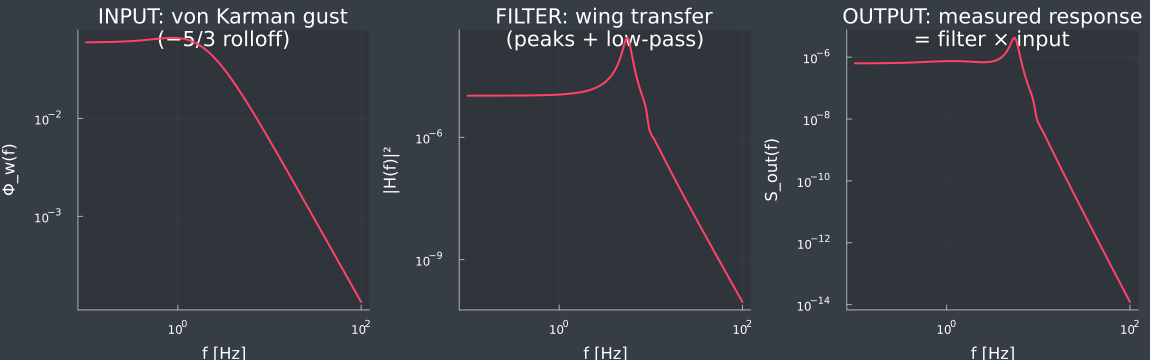
\includegraphics[width=\textwidth]{vonkarman_response.png}}
  {\fbox{\parbox{0.9\textwidth}{\centering\vspace{2em}
   \textit{Run} \texttt{vonkarman\_response.jl} \textit{to generate this figure
   (\texttt{vonkarman\_response.png}), then recompile.}\vspace{2em}}}}
\caption{Input, filter, and output. \textbf{Left:} the von K\'arm\'an gust PSD,
falling at the $-5/3$ slope. \textbf{Centre:} the squared transfer function
$|\mathbf H(f)|^2$---flat at low frequency, two resonant peaks at the natural
frequencies, and then a low-pass roll-off. \textbf{Right:} the measured output $S_{\text{out}}=|H|^2\Phi_w$, whose steep slope combines both
effects (left $\times$ middle $=$ right). The middle panel is the isolated structural filter and is obtained from the right
panel by spectral division \eqref{eq:divide}.}
\label{fig:result}
\end{figure}
\begin{description}
  \item[\textbf{Input} $\Phi_w(f)$:] The gust spectrum is flat below the knee
near $f\approx U/(2\pi L_w)$ and then decays at $-5/3$. This is the forcing received by the
wing and is independent of the wing's dynamics.
  \item[\textbf{Filter} $|H(f)|^2$:] The wing's intrinsic behaviour. Flat (quasi-static
        following) at low frequency; sharp resonance at $\omega_h$ and $\omega_\theta$
        from \eqref{eq:wn}; a $-4$ roll-off (corresponding to a $-2$ slope in $|\mathbf H|$) above the peaks because inertia cannot follow fast gusts. This panel therefore represents the ``low-pass with low-frequency resonance'' result.
  \item[\textbf{Output} $S_{\text{out}}(f)$:] Represents what an accelerometer on the wing would record. It still shows the resonant peaks, but its roll-off ($\approx\!-5.7$) is steeper
than the filter's because the input was already falling.
\end{description}

\begin{table}[ht]
\centering
\caption{Illustrative parameters (chosen to give two well-separated peaks).}
\label{tab:params}
\begin{tabular}{llll}
\toprule
Symbol & Value & Symbol & Value\\
\midrule
$m$ & $2.0$ kg & $\rho$ & $1.225$ kg/m$^3$\\
$I_p$ & $0.01$ kg\,m$^2$ & $U$ & $12$ m/s\\
$S$ & $0.015$ kg\,m & $c_{\text{chord}}$ & $0.30$ m\\
$k$ (each) & $1200$ N/m & $b_{\text{span}}$ & $0.50$ m\\
$c$ (each) & $3.0$ N\,s/m & $C_{l\alpha}$ & $2\pi$\\
$d$ & $0.25$ m & $e_a$ & $0.05$ m\\
$\sigma_w$ & $1.5$ m/s & $L_w$ & $1.0$ m\\
\bottomrule
\end{tabular}
\end{table}

\section{Time-Domain Realisation of the Gust Response}
\label{sec:time}

The frequency-domain results in the main text describe the response in a statistical,
steady-state sense. To visualise the same behaviour as an explicit time history, we (i)
synthesise a single random gust signal whose power spectral density (PSD) matches the von
K\'arm\'an model of Eq.~\eqref{eq:vk-time}, and (ii) integrate the equations of motion
\eqref{eq:eom} forward in time. All parameters are identical to those of
Table~\ref{tab:params}.

\subsection{Synthesising the Gust Signal}
A random signal with a prescribed PSD is generated using the \emph{spectral
representation} (random-phase) method. The record has $N$ samples at sampling rate $f_s$,
so the discrete one-sided frequencies are $f_n=n f_s/N$ with $\omega_n=2\pi f_n$. At each
frequency, we assign the von K\'arm\'an amplitude and an independent random phase
$\phi_n\sim\mathcal U(0,2\pi)$:
\begin{equation}
\hat W_n=\sqrt{\tfrac{N f_s}{2}\,S_f(f_n)}\;e^{\,i\phi_n},
\qquad
S_f(f)=2\,(2\pi)\,\Phi_w(\omega),
\label{eq:synth}
\end{equation}
where $\Phi_w(\omega)$ is the temporal PSD of Eq.~\eqref{eq:vk-time}; the factor $2\pi$
converts the density from per-rad/s to per-Hz, and the factor $2$ converts the two-sided
density to a one-sided one. The time signal is the inverse real FFT,
\begin{equation}
w_g(t_j)=\mathrm{IFFT}\{\hat W_n\}, \qquad t_j=j/f_s,
\end{equation}
after which it is rescaled so that its sample standard deviation equals the target intensity
$\sigma_w$. Finally, a small broadband component (here $2\%$ of $\sigma_w$) is added to
represent measurement noise:
\begin{equation}
w_g\;\leftarrow\;w_g+0.02\,\sigma_w\,\eta(t),\qquad \eta\sim\mathcal N(0,1).
\end{equation}
Because the phases are random, each run produces a different but statistically equivalent
gust; by construction, its expected PSD is exactly $\Phi_w$.

\subsection{Integrating the Equations of Motion}
Equation~\eqref{eq:eom} is recast in first-order state-space form with state
$\mathbf x=[\,h,\ \theta,\ \dot h,\ \dot\theta\,]^{\mathsf T}$:
\begin{equation}
\dot{\mathbf x}=\mathbf A\,\mathbf x+\mathbf B\,w_g,\qquad
\mathbf A=\begin{bmatrix}\mathbf 0 & \mathbf I\\[2pt]
-\mathbf M^{-1}(\mathbf K_s+\mathbf K_a) & -\mathbf M^{-1}(\mathbf C+\mathbf C_a)\end{bmatrix},\qquad
\mathbf B=\begin{bmatrix}\mathbf 0\\[2pt]\mathbf M^{-1}\mathbf F_g\end{bmatrix}.
\label{eq:ss}
\end{equation}
Since the gust is sampled at the fixed step $\Delta t=1/f_s$, we treat it as constant over
each step (zero-order hold), for which the state update is \emph{exact}:
\begin{equation}
\mathbf x_{j+1}=\mathbf A_d\,\mathbf x_j+\mathbf B_d\,w_g(t_j),\qquad
\mathbf A_d=e^{\mathbf A\Delta t},\qquad
\mathbf B_d=\mathbf A^{-1}\!\big(\mathbf A_d-\mathbf I\big)\mathbf B.
\label{eq:zoh}
\end{equation}
Using the matrix exponential avoids the accuracy and stability limitations of a simple
explicit time-stepper, which matters here because the lightly damped resonances would
otherwise require a very small time step.

\subsection{Reading the Time History}
Figure~\ref{fig:time} shows a representative 10-second window of the gust together with the
resulting plunge $h(t)$ and pitch $\theta(t)$. The physical content of the main result is
visible as a difference in character between the panels:
\begin{itemize}
  \item The \textbf{gust} (top) is jagged and broadband: turbulence carries energy across a
        wide range of frequencies, including rapid fluctuations.
  \item The \textbf{plunge} response (middle) is markedly smoother and more periodic. The
        high-frequency content of the gust has been attenuated (the low-pass action), while
        the motion is dominated by oscillation near the plunge natural frequency
        $\omega_h$ of Eq.~\eqref{eq:wn} (the resonance).
  \item The \textbf{pitch} response (bottom) contains more high-frequency content than the plunge because its natural
        frequency $\omega_\theta$ is higher and the two modes are inertially coupled, so it
        retains comparatively more high-frequency energy --- consistent with the pitch
        transfer function exhibiting both peaks in Fig.~\ref{fig:result}.
\end{itemize}
In short, a rough, broadband input produces a smooth, resonant output: the time-domain
counterpart of the low-pass-with-resonance transfer function. The root-mean-square response
levels (plunge $\approx 11$~mm, pitch $\approx 1.8^\circ$ for the parameters used) provide a
quantitative measure of the gust loading.

\begin{figure}[ht]
\centering
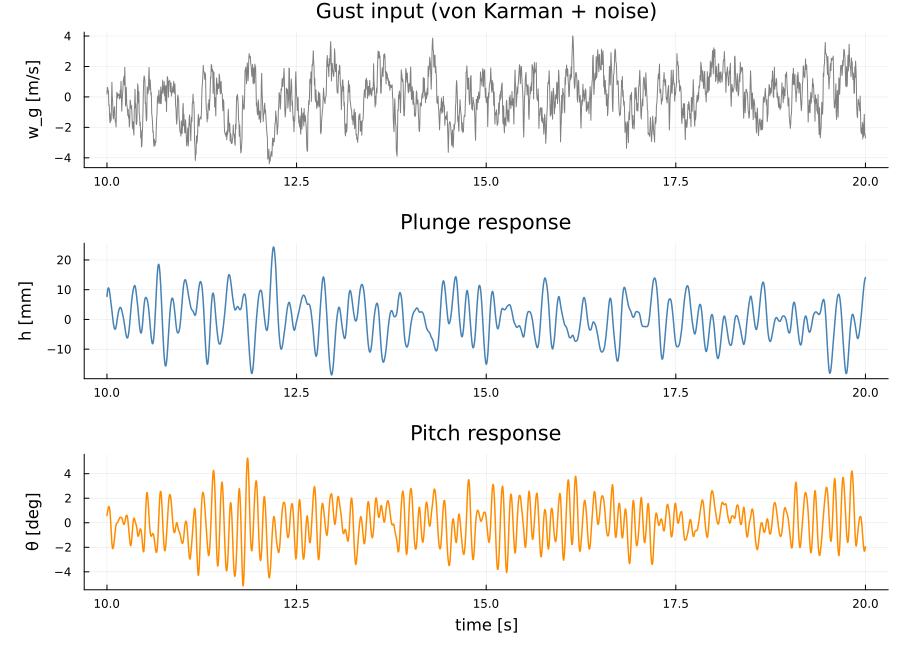
\includegraphics[width=0.92\textwidth]{vonkarman_timedomain.png}
\caption{One realisation of the random gust (top) and the resulting wing motion: plunge
(middle) and pitch (bottom). The smoothing and near-periodic character of the response,
relative to the broadband input, are the time-domain signature of the wing's low-pass
filtering and resonance.}
\label{fig:time}
\end{figure}

\paragraph{Consistency Check.} Estimating the PSD of the simulated $h(t)$ (e.g., by Welch's
method) and dividing by the gust PSD recovers $|H_h(i\omega)|^2$, reproducing the middle
panel of Fig.~\ref{fig:result} to within the statistical scatter of a finite record. This
closes the loop between the time-domain realisation and the analytical transfer function.

\paragraph{Caveat.} The absolute response amplitudes depend on the quasi-steady aerodynamic
assumption, which omits unsteady aerodynamic damping and therefore somewhat overpredicts the
resonant motion. The qualitative result --- broadband input, smooth resonant output --- is
independent of this assumption.

%======================================================================
\section{Limitations}
%======================================================================
The aerodynamics are quasi-steady: lift responds instantaneously to the effective angle of attack 
(including kinematic velocities). While this captures the primary aerodynamic damping, 
it omits the unsteady wake memory effects and phase lags captured by Theodorsen's and Sears' functions. This tends to overpredict peak height but does not change the qualitative low-pass-plus-resonance
shape. Furthermore, the quasi-steady aerodynamic model used here omits the kinematic vertical velocity induced at the aerodynamic centre by the pitch rate ($-e_a \dot{\theta}$), a common simplification that isolates the primary plunge-damping mechanism but slightly underestimates the total aerodynamic damping.

The single rigid section also has no spanwise bending modes; it represents one
characteristic section rather than a full flexible wing. Both simplifications are standard at
this level of analysis and are appropriate for demonstrating the filtering mechanism.

% =====================================================================
\section{Conclusion}
% =====================================================================
A wing buffeted by turbulence behaves as a low-pass filter with resonant peaks
at its low natural frequencies. A two-degree-of-freedom typical section, forced
by a von K\'arm\'an gust and analysed through its transfer function,
demonstrates this mechanism clearly and efficiently without resolving the turbulent flow. The essential subtlety is that the measured response spectrum blends the
structure's filtering with the input's own shape; only the transfer function,
recovered by spectral division, isolates the structural behaviour that the study
set out to characterise.

\appendix
\begin{appendices}

\section{The Dryden Gust Model and Response}
\label{app:dryden}

The von K\'arm\'an spectrum of Eq.~\eqref{eq:vk-time} contains the fractional power $11/6$,
which makes it inconvenient to realise as a rational forming filter. The \emph{Dryden} model
is the standard rational approximation: it matches von K\'arm\'an at low frequency and in
total energy, but uses integer powers. This appendix repeats the spectral and time-domain
analysis using Dryden turbulence; all structural and aerodynamic parameters are unchanged
(Table~\ref{tab:params}).

\subsection{Dryden Spectrum}
The MIL-F-8785C Dryden vertical-gust PSD, as a function of spatial frequency $\Omega$, is
\begin{equation}
\Phi_w(\Omega)=\sigma_w^2\,\frac{L_w}{\pi}\,
\frac{1+3\,(L_w\Omega)^2}{\big[\,1+(L_w\Omega)^2\,\big]^{2}} .
\label{eq:dryden-space}
\end{equation}
Applying the same frozen-turbulence change of variable as in the main text
($\Omega=\omega/U$, density scaled by $1/U$) gives the temporal spectrum
\begin{equation}
\boxed{\;\Phi_w(\omega)=\frac{\sigma_w^2 L_w}{\pi U}\,
\frac{1+3\,(L_w\,\omega/U)^2}{\big[\,1+(L_w\,\omega/U)^2\,\big]^{2}}\;}
\label{eq:dryden-time}
\end{equation}
At high frequency, the numerator grows like $\omega^2$ and the denominator like $\omega^4$, so
\begin{equation}
\Phi_w(\omega)\sim\omega^{-2},
\end{equation}
a steeper roll-off than the von K\'arm\'an value of $\omega^{-5/3}$. Physically, Dryden
under-represents the very-high-frequency turbulent energy; the two models are
nearly indistinguishable across the low-frequency band that contains the wing's resonances,
which is why either is acceptable for this study.

\subsection{Forming-Filter Interpretation}
A practical advantage of \eqref{eq:dryden-time} is that it factorises. Driving unit-intensity
white noise $\eta$ through the linear filter
\begin{equation}
G_w(s)=\sigma_w\sqrt{\frac{L_w}{\pi U}}\,
\frac{1+\sqrt{3}\,(L_w/U)\,s}{\big[\,1+(L_w/U)\,s\,\big]^{2}}
\label{eq:dryden-filter}
\end{equation}
produces a signal whose PSD is exactly \eqref{eq:dryden-time}, since
$|G_w(i\omega)|^2=\Phi_w(\omega)$. This is the form used in real-time flight simulators.
For consistency with Section~\ref{sec:time}, the realisation here instead uses the same
random-phase spectral-synthesis method, simply substituting \eqref{eq:dryden-time} for the
target PSD; both routes are statistically equivalent.

\subsection{Spectral Response}
The gust-to-response transfer function $\mathbf H(i\omega)$ of Eq.~\eqref{eq:H} depends only
on the structure and aerodynamics, \emph{not} on the turbulence model. The middle panel of
Fig.~\ref{fig:dryden-spec} is therefore identical to that of Fig.~\ref{fig:result}; only the
input spectrum, and consequently the output $S_{\text{out}}=|H_h|^2\Phi_w$, differ. The
output now rolls off as $\omega^{-2}\!\cdot\!\omega^{-4}=\omega^{-6}$.

\begin{figure}[ht]
\centering
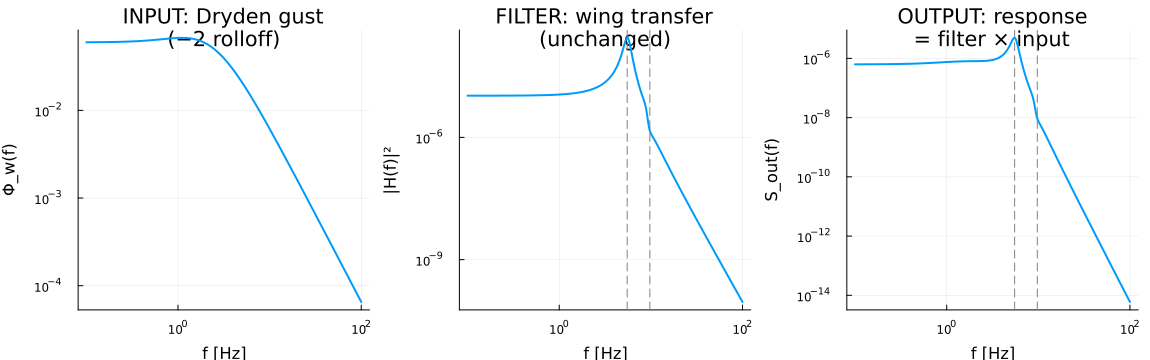
\includegraphics[width=\textwidth]{dryden_response.png}
\caption{Dryden input spectrum (left, $-2$ slope), the unchanged wing transfer function
(middle), and the resulting output spectrum (right). Compare with the von K\'arm\'an result
in Fig.~\ref{fig:result}: the resonance peaks sit at the same frequencies; only the
high-frequency slope of the input and output differs.}
\label{fig:dryden-spec}
\end{figure}

\subsection{Time-Domain Response}
A random Dryden gust is synthesised and integrated exactly as in Section~\ref{sec:time}
(Eqs.~\eqref{eq:synth}--\eqref{eq:zoh}). Figure~\ref{fig:dryden-time} shows a representative
window. As before, the broadband gust produces a smoother, near-periodic wing motion
dominated by the natural frequencies --- the same low-pass-plus-resonance behaviour. The
RMS response levels (plunge $\approx 12$~mm, pitch $\approx 1.8^\circ$) are within a few
percent of the von K\'arm\'an values, confirming that the choice of turbulence model has only
a minor effect on the structural response for this configuration.

\begin{figure}[ht!]
\centering
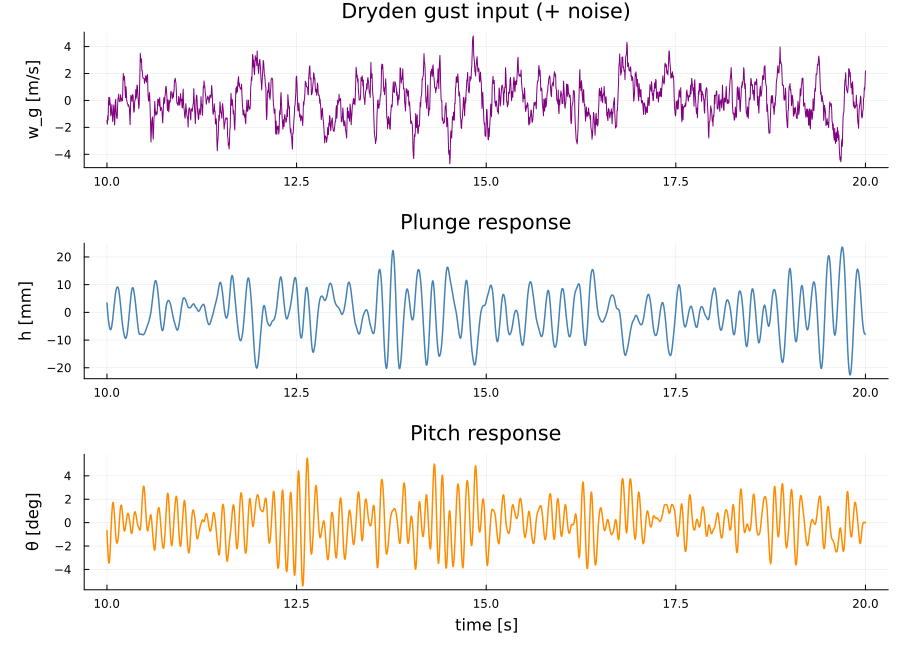
\includegraphics[width=0.75\textwidth]{dryden_timedomain.png}
\caption{One realisation of a Dryden gust (top) and the resulting plunge (middle) and pitch
(bottom) response. The result is visually and quantitatively close to the von K\'arm\'an case
of Fig.~\ref{fig:time}.}
\label{fig:dryden-time}
\end{figure}

\section{Multisine Excitation for Structural Identification}
\label{app:multisine}

The von K\'arm\'an and Dryden analyses (Section~\ref{sec:time} and Appendix~\ref{app:dryden})
use \emph{random} gusts to reproduce realistic turbulent loading. For \emph{structural
identification} --- extracting the natural frequencies, damping, and the transfer function
itself --- a deterministic excitation is preferable. This appendix uses a \textbf{multisine}:
a sum of sinusoids at chosen frequencies, containing no random noise. All structural and
aerodynamic parameters are unchanged (Table~\ref{tab:params}).

\subsection{Multisine Definition}
The excitation is
\begin{equation}
w_g(t)=\sum_{j=1}^{K} A_j \sin\!\big(2\pi f_j t+\phi_j\big),
\qquad f_j = j\,f_0,
\label{eq:multisine}
\end{equation}
with the following design choices:
\begin{itemize}
  \item \textbf{Harmonic frequencies} $f_j=j f_0$. Choosing the base frequency
        $f_0=1/T_{\text{per}}$ makes $w_g$ exactly periodic with period $T_{\text{per}}$;
        analysing an integer number of periods then gives \emph{leakage-free} spectra. Here,
        $f_0=0.25$~Hz with $j=1\ldots80$ spans $0.25$--$20$~Hz, bracketing both resonances.
  \item \textbf{Flat amplitude} $A_j=\sigma_w\sqrt{2/K}$, so every frequency in the band is
        excited equally and $w_g$ has the prescribed RMS $\sigma_w$.
  \item \textbf{Schroeder phases} $\phi_j=-\,\pi j(j-1)/K$, which minimise the
        \emph{crest factor} (peak-to-RMS ratio). A low crest factor keeps the signal within
        amplitude limits while delivering maximum energy; here the crest factor is $\approx1.9$.
\end{itemize}
The integration of Eq.~\eqref{eq:eom} is performed exactly as in Section~\ref{sec:time}
(zero-order-hold, Eqs.~\eqref{eq:ss}--\eqref{eq:zoh}).

\subsection{Leakage-Free Transfer-Function Estimate}
Because the input is periodic and noise-free, the steady-state response is periodic with the
same period. Taking the discrete Fourier transform of a single steady period of input and
output, the transfer function at each excited line is obtained directly as the ratio of
Fourier coefficients,
\begin{equation}
\hat H(f_j)=\frac{\mathcal F\{h\}(f_j)}{\mathcal F\{w_g\}(f_j)} .
\label{eq:frf-est}
\end{equation}
Unlike a windowed estimate from a random signal, \eqref{eq:frf-est} carries \emph{no spectral
leakage and no statistical variance}: it reproduces the analytical transfer function
\eqref{eq:H} to within the (negligible) discretisation error. The middle panel of
Fig.~\ref{fig:multisine-spec} shows the measured points lying exactly on the analytical curve,
including through the two resonance peaks --- this is the property that makes multisine
excitation the standard tool for experimental modal analysis and frequency-response
identification.

\begin{figure}[ht]
\centering
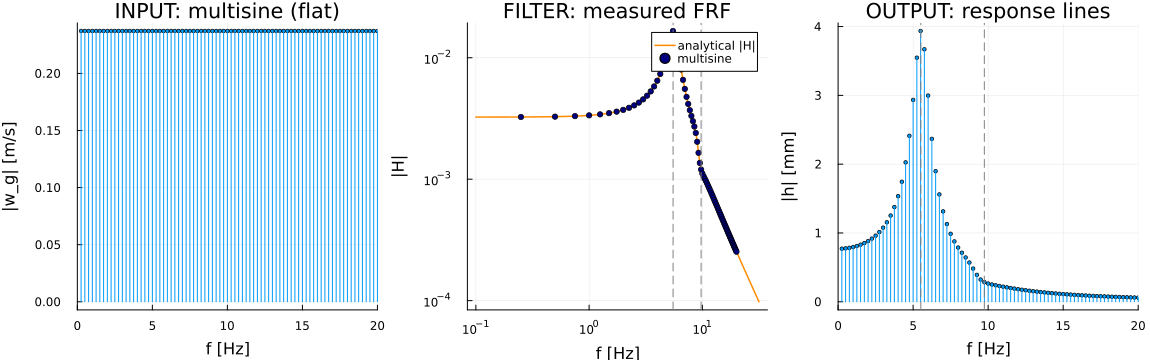
\includegraphics[width=\textwidth]{multisine_response.png}
\caption{Multisine structural analysis. Left: the flat-amplitude line spectrum of the input.
Middle: the transfer function recovered from the simulation (markers) lies exactly on the
analytical $|H(f)|$ (line); dashed lines mark the plunge and pitch natural frequencies.
Right: the response line spectrum, peaking sharply at the resonances.}
\label{fig:multisine-spec}
\end{figure}

\subsection{Time-Domain Response}
Figure~\ref{fig:multisine-time} shows two steady-state periods of the excitation and response.
The Schroeder phasing gives the input a swept (chirp-like) appearance within each period, and
the two periods are identical --- the deterministic, repeatable character that distinguishes
this case from the random gusts. The response exhibits pronounced \emph{bursts} of large
amplitude precisely when the instantaneous excitation frequency passes through a natural
frequency: the earlier burst corresponds to the plunge resonance, the later (higher-frequency)
burst to the pitch resonance. This is the same low-pass-with-resonance behaviour seen
throughout, now displayed as a controlled frequency sweep rather than a stochastic record.

\begin{figure}[ht!]
\centering
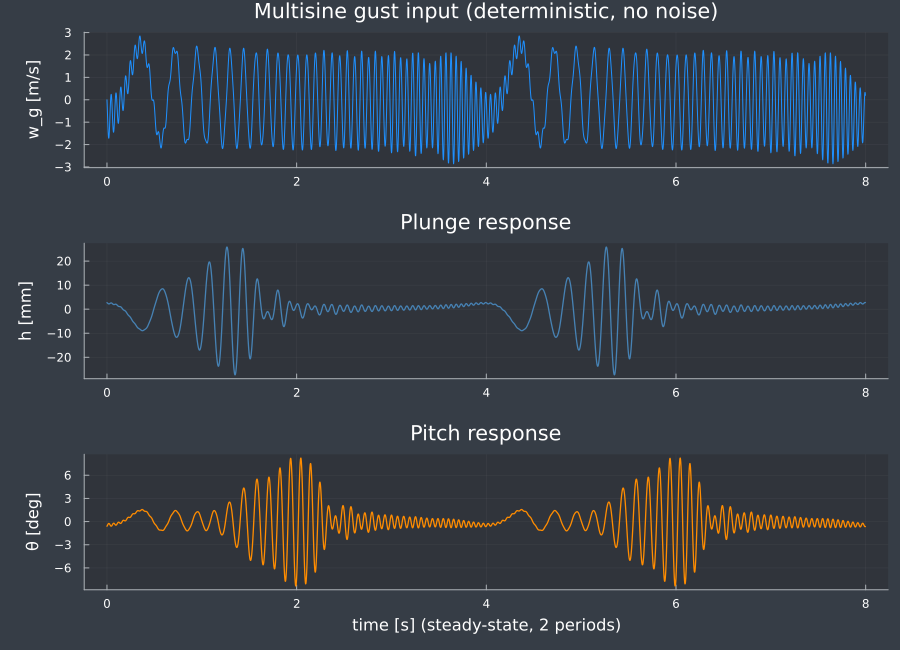
\includegraphics[width=0.92\textwidth]{multisine_timedomain.png}
\caption{Two steady-state periods of the multisine gust (top) and the resulting plunge
(middle) and pitch (bottom) response. Large-amplitude bursts occur as the swept frequency
crosses each resonance; the exact repetition between periods reflects the deterministic,
noise-free nature of the excitation.}
\label{fig:multisine-time}
\end{figure}

\subsection{When to Use Which Excitation}
The random (von K\'arm\'an, Dryden) and deterministic (multisine) approaches are
complementary. The random gusts answer \emph{``how does the wing respond to realistic
turbulence?''} and yield response statistics such as RMS levels. The multisine answers
\emph{``what is the wing's transfer function, and where are its modes?''} and yields a clean,
repeatable frequency-response measurement. Together they cover both the realistic-loading and
the system-identification aspects of the same model.

\end{appendices}
% =====================================================================
\newpage
\bibliographystyle{plain} % We choose the "plain" reference style
\bibliography{refs} % Entries are in the refs.bib file
\end{document}
